%% Begin slides template file
\documentclass[11pt,t,usepdftitle=false,aspectratio=169]{beamer}
%% ------------------------------------------------------------------
%% - aspectratio=43: Set paper aspect ratio to 4:3.
%% - aspectratio=169: Set paper aspect ratio to 16:9.
%% ------------------------------------------------------------------
\usepackage{graphicx}
\usepackage{hyperref}
\usetheme[nototalframenumber,logo,license]{uibk}

%% NOTES
\usepackage{pgfpages}
\setbeameroption{show notes on second screen=right} % Both

\usepackage[]{natbib}

%% ------------------------------------------------------------------
%% - foot: Add a footer line for conference name and date.
%% - logo: Add the university logo in the footer (only if 'foot' set).
%% - bigfoot/sasquatch: Larger font size in footer.
%% - nototalslidenumber: Hide the total number of slides (only if 'foot' set)
%% - license: Add CC-BY license symbol to title slide (e.g., for conference uploads)
%%   (TODO: At the moment no other licenses are supported.)
%% - licenseall: Add CC-BY license symbol to all subsequent slides slides
%% - url: use \url{} rather than \href{} on the title page
%% ------------------------------------------------------------------

%% ------------------------------------------------------------------
%% The official corporate colors of the university are predefined and
%% can be used for e.g., highlighting something. Simply use
%% \color{uibkorange} or \begin{color}{uibkorange} ... \end{color}
%% Defined colors are:
%% - uibkblue, uibkbluel, uibkorange, uibkorangel, uibkgray, uibkgraym, uibkgrayl
%% The frametitle color can be easily adjusted e.g., to black with
%% \setbeamercolor{titlelike}{fg=black}
%% ------------------------------------------------------------------

%\setbeamercolor{verbcolor}{fg=uibkorange}
%% ------------------------------------------------------------------
%% Setting a highlight color for verbatim output such as from
%% the commands \pkg, \email, \file, \dataset
%% ------------------------------------------------------------------


%% information for the title page ('short title' is the pdf-title that is shown in viewer's titlebar)
\title[IoT Light Bulb Attack]{IoT Light Bulb Covert Channel}
\subtitle{Extended Functionality Attack on Smart Lights}
\URL{}

\author[Julia Wanker \& Bennett Piater]{Julia Wanker, Bennett Piater}
%('short author' is the pdf-metadata Author)
%% If multiple authors are required and the font size is too large you
%% can overrule the font size of author and url by calling:
%\setbeamerfont{author}{size*={10pt}{10pt},series=\mdseries}
%\setbeamerfont{url}{size*={10pt}{10pt},series=\mdseries}
%\URL{}
%\subtitle{}

\footertext{}
\date{2018-06-14}

\headerimage{3}
%% ------------------------------------------------------------------
%% The theme offers four different header images based on the
%% corporate design of the university of innsbruck. Currently
%% 1, 2, 3 and 4 is allowed as input to \headerimage{...}. Default
%% or fallback is '1'.
%% ------------------------------------------------------------------

\begin{document}

%% ALTERNATIVE TITLEPAGE
%% The next block is how you add a titlepage with the 'nosectiontitlepage' option, which switches off
%% the default behavior of creating a titlepage every time a \section{} is defined.
%% Then you can use \section{} as it's originally intended, including a table of contents.
% \usebackgroundtemplate{\includegraphics[width=\paperwidth,height=\paperheight]{titlebackground.pdf}}
% \begin{frame}[plain]
%     \titlepage
% \end{frame}
% \addtocounter{framenumber}{-1}
% \usebackgroundtemplate{}}

%% Table of Contents, if wanted:
%% this requires the 'nosectiontitlepage' option and setting \section{}'s as you want them to appear here.
%% Subsections and subordinates are suppressed in the .sty at the moment, search
%% for \setbeamertemplate{subsection} and replace the empty {} with whatever you want.
%% Although it's probably too much for a presentation, maybe for a lecture.
% \begin{frame}
%     \vspace*{1cm plus 1fil}
%     \tableofcontents
%     \vspace*{0cm plus 1fil}
% \end{frame}

%%%%%%%%%%%%%%%%%%%%%%%%%%%%%%%%%%%%%%%%%%%%%%%%%%%%%%%%%%%%%%%%%%%%%%%%%
% Intro:
% - names
% - topic
% - structure: First Taxonomy (main paper), then overview of main paper and possible related work
%%%%%%%%%%%%%%%%%%%%%%%%%%%%%%%%%%%%%%%%%%%%%%%%%%%%%%%%%%%%%%%%%%%%%%%%%


\section{Topic Relevance} % 2 min
\label{sec:relevance}
\title{Topic Relevance}
\subtitle{New Attack Vectors on IoT Devices}

\subsection{IoT Security in General} % 1 min
\label{sub:general_security}
\begin{frame}{IoT Security in General} % talk about security challenges which arise with iot
	\only<1>
	{
		\begin{figure}
			\centering
			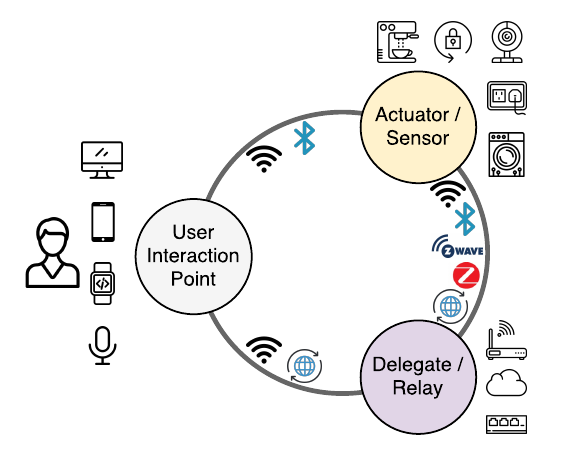
\includegraphics[height=5.5cm,keepaspectratio]{img/iot_ecosystem.png}
			\caption{\small{Infrastructure of IoT ecosystem} \footnote{\tiny{Zhan et. al. Understanding IoT Security Through the Data Crystal Ball: Where We Are Now and Where We Are Going to Be}}}
		\end{figure}
		
	}
	\only<2> % attack vectors 
	{
		\begin{figure}
			\centering
			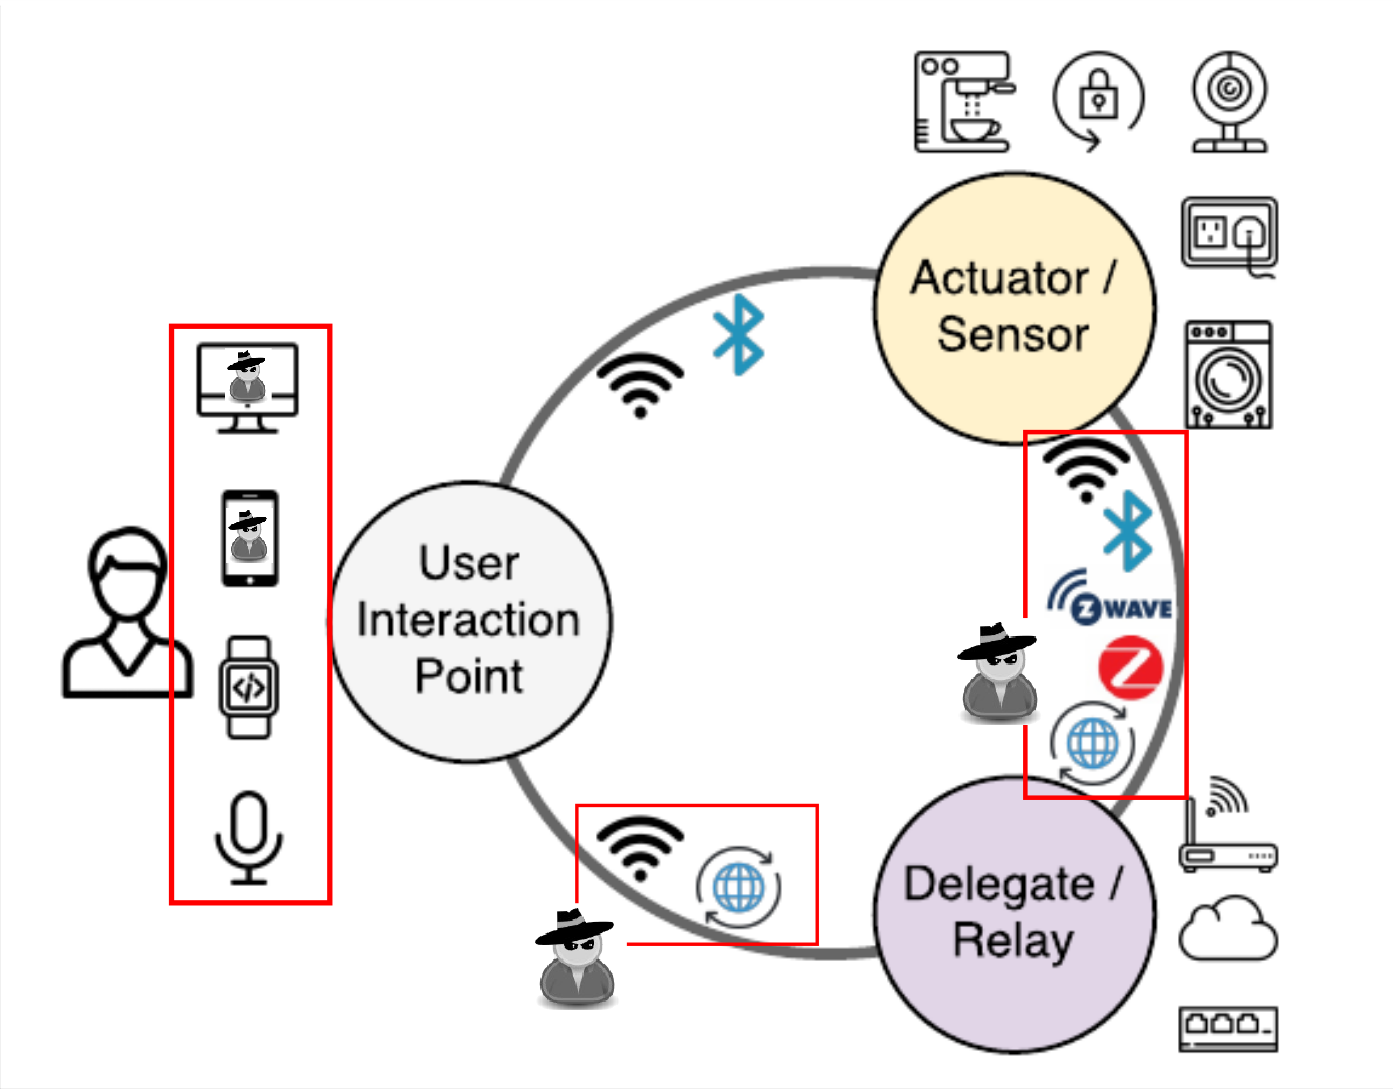
\includegraphics[height=5.5cm, keepaspectratio]{img/iot-ecosystem_attack-vectors.png}
			\caption{\small{Attack Vectors in IoT ecosystem} \footnote{\tiny{Zhan et. al. Understanding IoT Security Through the Data Crystal Ball: Where We Are Now and Where We Are Going to Be / \textit{edited}}}}
		\end{figure}
	}
\end{frame}

\subsection{Smart Light Security} % .5 min
\label{sub:smart_light_security}
\begin{frame}{Smart Light Security} % talk about importance of focus on smart light security (-> ubiquity) --> name example of zll worm (IoT goes nuclear paper)
	\begin{figure} % TODO: QUESTION: since we just shortly introduce smart light security here (I would do this with the example of the IoT goes nuclear paper), I chose this pictur - not 100% sure if it is suitable - what do you think ?
		\centering
		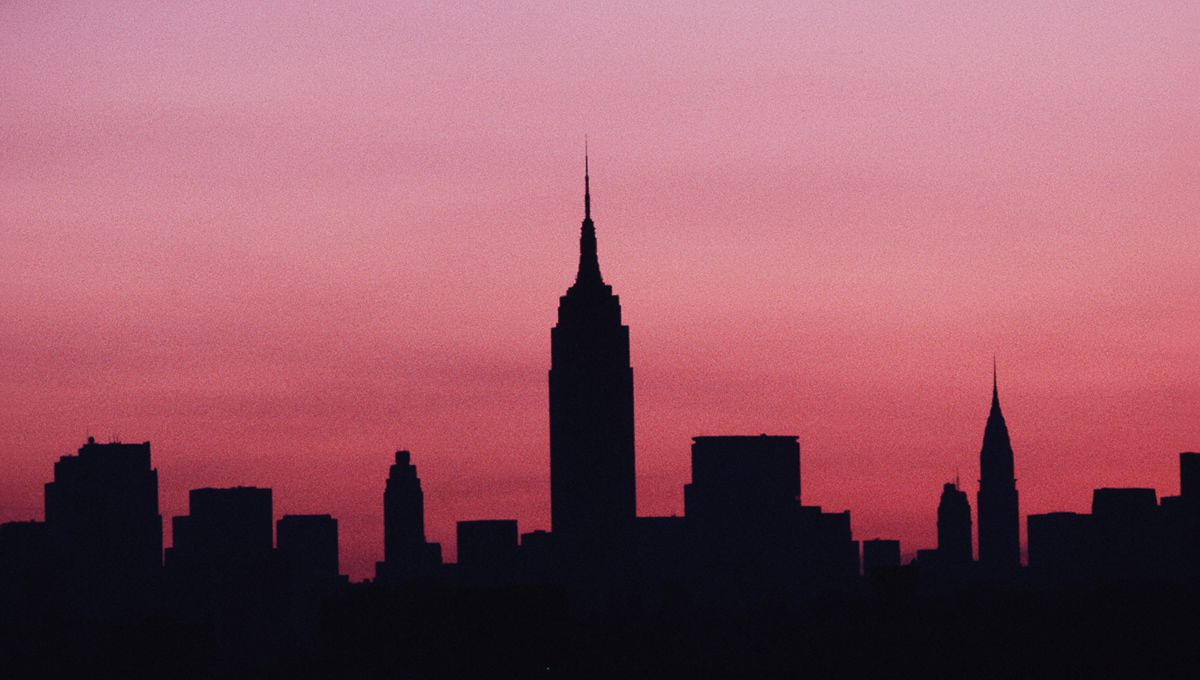
\includegraphics{img/nyc-blackout.jpg}
		\caption{\small{NYC Blackout of 1977 (Allan Tannenbaum/Getty Images)}}
	\end{figure}
\end{frame}

\subsubsection{Extending Functionality} % .5 min
\label{subsub:extending}
\begin{frame}{Extending Functionality} % give reminder that we focus on covert data transmission over smart lights
	\begin{figure}
		\centering
		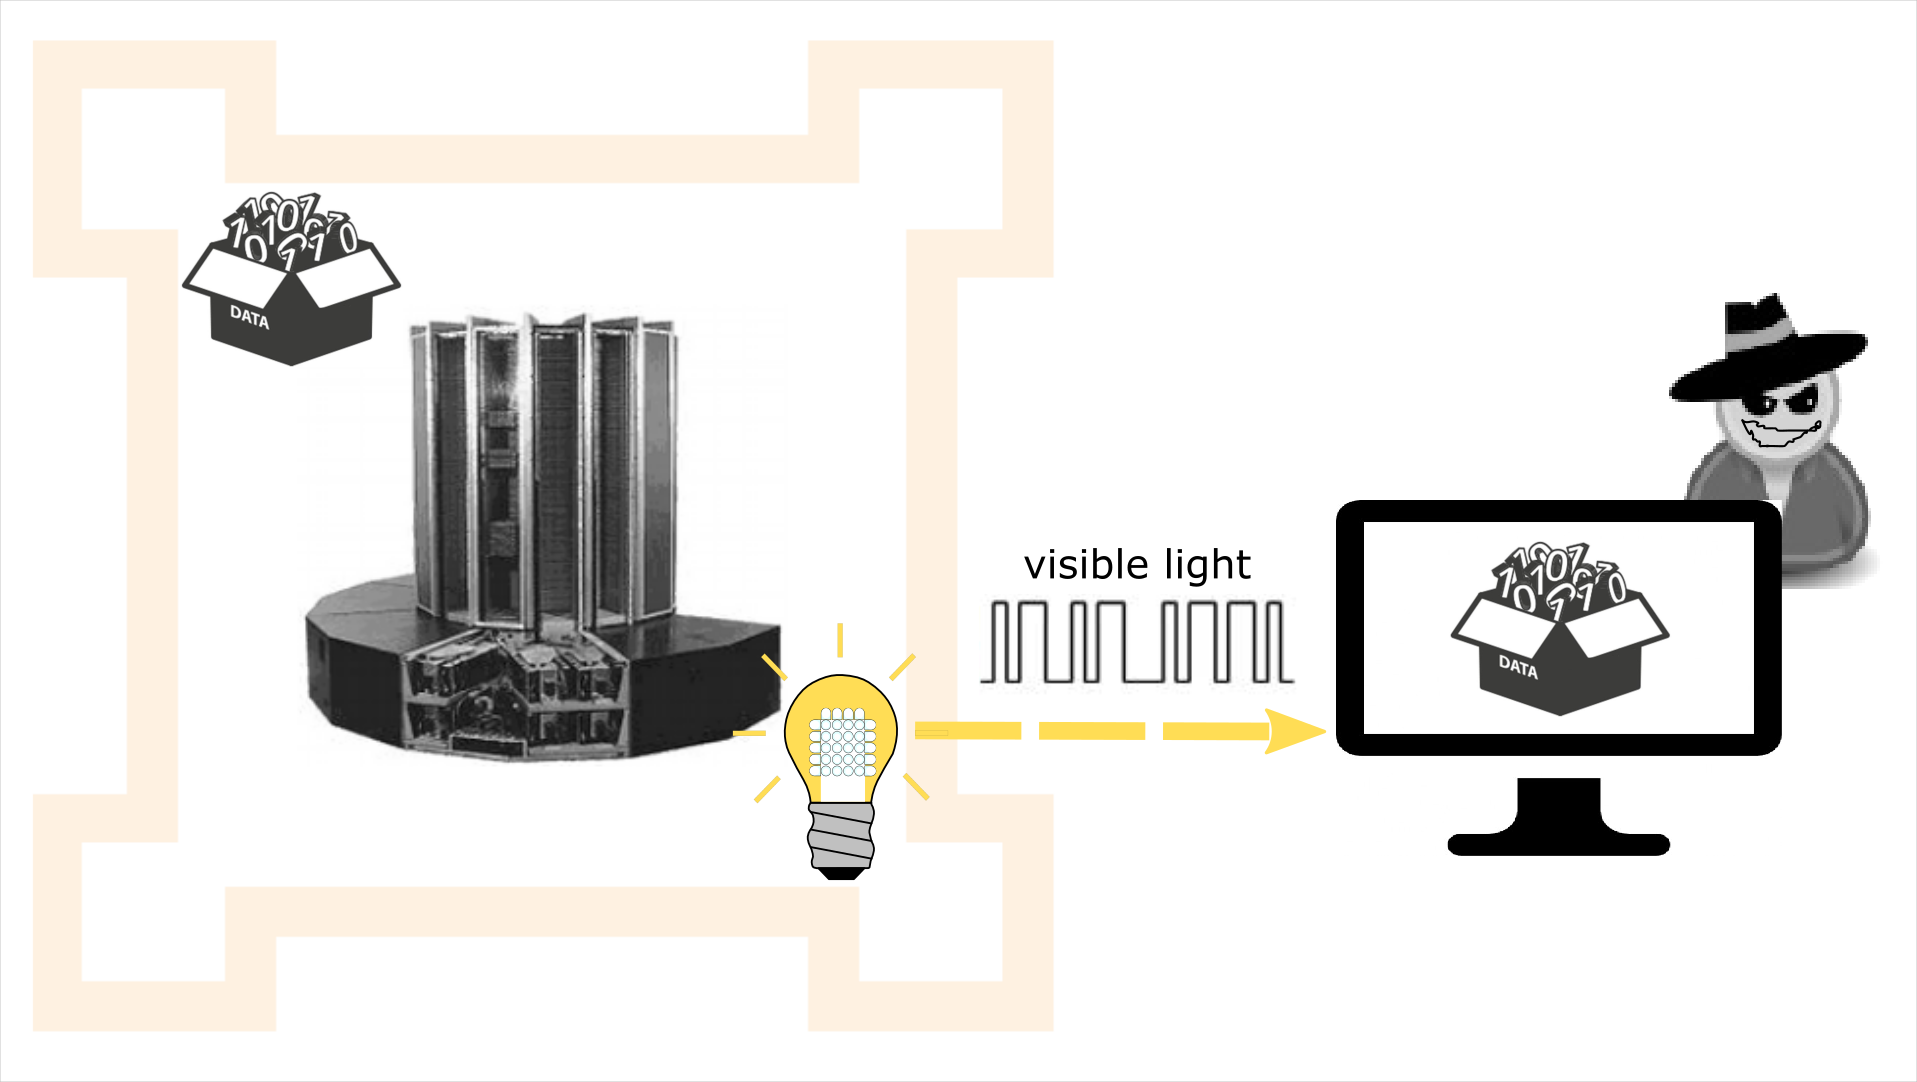
\includegraphics{img/extended-func-attack-light.png}
	\end{figure}
\end{frame}


\section{Theoretical Background} % 3 min
\label{sec:theory}
\title{Theoretical Background} 
\subtitle{Extended Functionality Attack on Smart Lights} % describe how communication with lights in general works and then how it is done with smart lights; name requirements in order to do that covertly (which more or less is standard since communication doesn't affect illumination)

\subsection{(Covert) Communication With Lights} % 1.5 min
\label{sub:covert_light_communication}
\begin{frame}{Communication With Lights}
	\begin{block}{General Light Communication}
		\begin{itemize}
			\item Change PWM signal
			\item \textbf{Off} period represents logical \textbf{0}
			\item \textbf{On} period represents logical \textbf{1}
		\end{itemize}
		
	\end{block}
	\begin{block}{Smart Light Communication}
		\begin{itemize}
			\item Send close brightness change commands
			\item \textbf{Lower leve} represents logical \textbf{0}
			\item \textbf{Higher level} represents logical \textbf{1}
		\end{itemize}
	\end{block}
\end{frame}
\begin{frame}{(Covert) Communication With Lights}
	\begin{block}{Covertness}
	\begin{itemize}
		\item Flicker at a rate above 60 Hz or use close brightness commands
		\item Detectable by sensor but not seen by human eye
	\end{itemize}
\end{block}
\end{frame}

\subsection{Smart Light Systems} % 1.5 min
\label{sub:smart_lights}
\begin{frame}{Smart Light Systems} % show components of smart light system, how component communicate 
  \begin{figure}
  	\centering
  	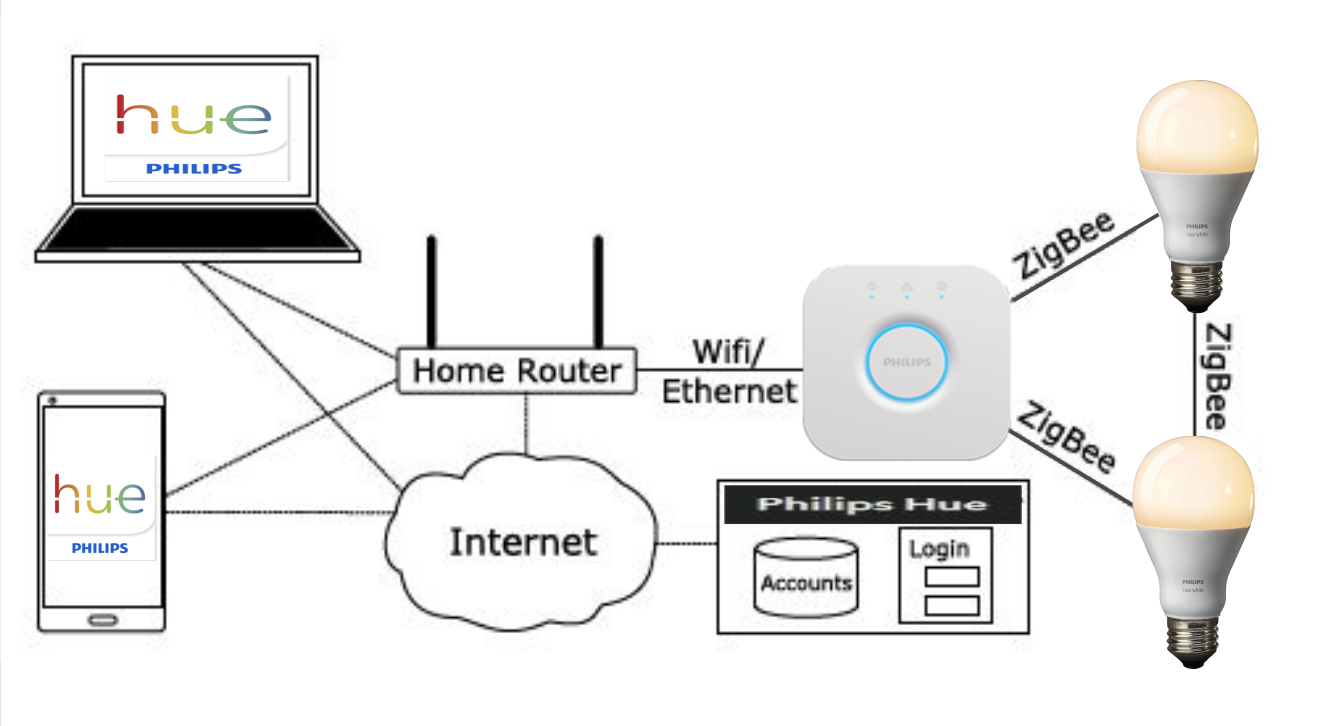
\includegraphics{img/smart-light-system.png} 
  	\caption{\small{System architecture of a Philips Hue connected lighting system with two bulbs} \footnote{\tiny{Morgner et al. All Your Bulbs Are Belong to Us: Investigating the Current State of Security in Connected Lighting Systems / \textit{edited}}}}
  \end{figure}
\end{frame}


\section{Experiment}%
\label{sec:experiment}

\subsection{Controlling the Light} % TODO: NOTE: I would mention how the communication in a smart light system works in the context of the smart light system setup (Theoretical Background - slide 6, before) - but regarding slides I would just leave it like this 'cause now we have a smooth leading over from Theoretical Background to Experiment section ?
\label{sub:controlling_the_lights}

\begin{frame}{Controlling the Light}
	We use the Hue API for simplicity.
	\begin{itemize}
		\item Bridge controls light via ZLL
		\item We interface with REST-API on bridge
	\end{itemize}

	\pause
	\begin{block}{Limitations}
		\begin{itemize}
			\item Rate limit due to throttling by bridge?
			\item Automatic fading by the bridge or light (no phase shifts!)
		\end{itemize}
		May be worked around some by speaking ZLL directly?
	\end{block}
\end{frame}

\subsection{Experimental Setup}%
\label{sub:experimental_setup}

\begin{frame}{Overview}
	% Diagramm:
	% - Arduino setzt Einstellungen vom Sensor
	% - Probe vom Pico hängt am Sensor und an der Masse/Erdung/Ground vom Arduino
	% - Arduino und Pico hängen am Laptop
	% - Python-Logo im Laptop
	\begin{figure}
		\centering
		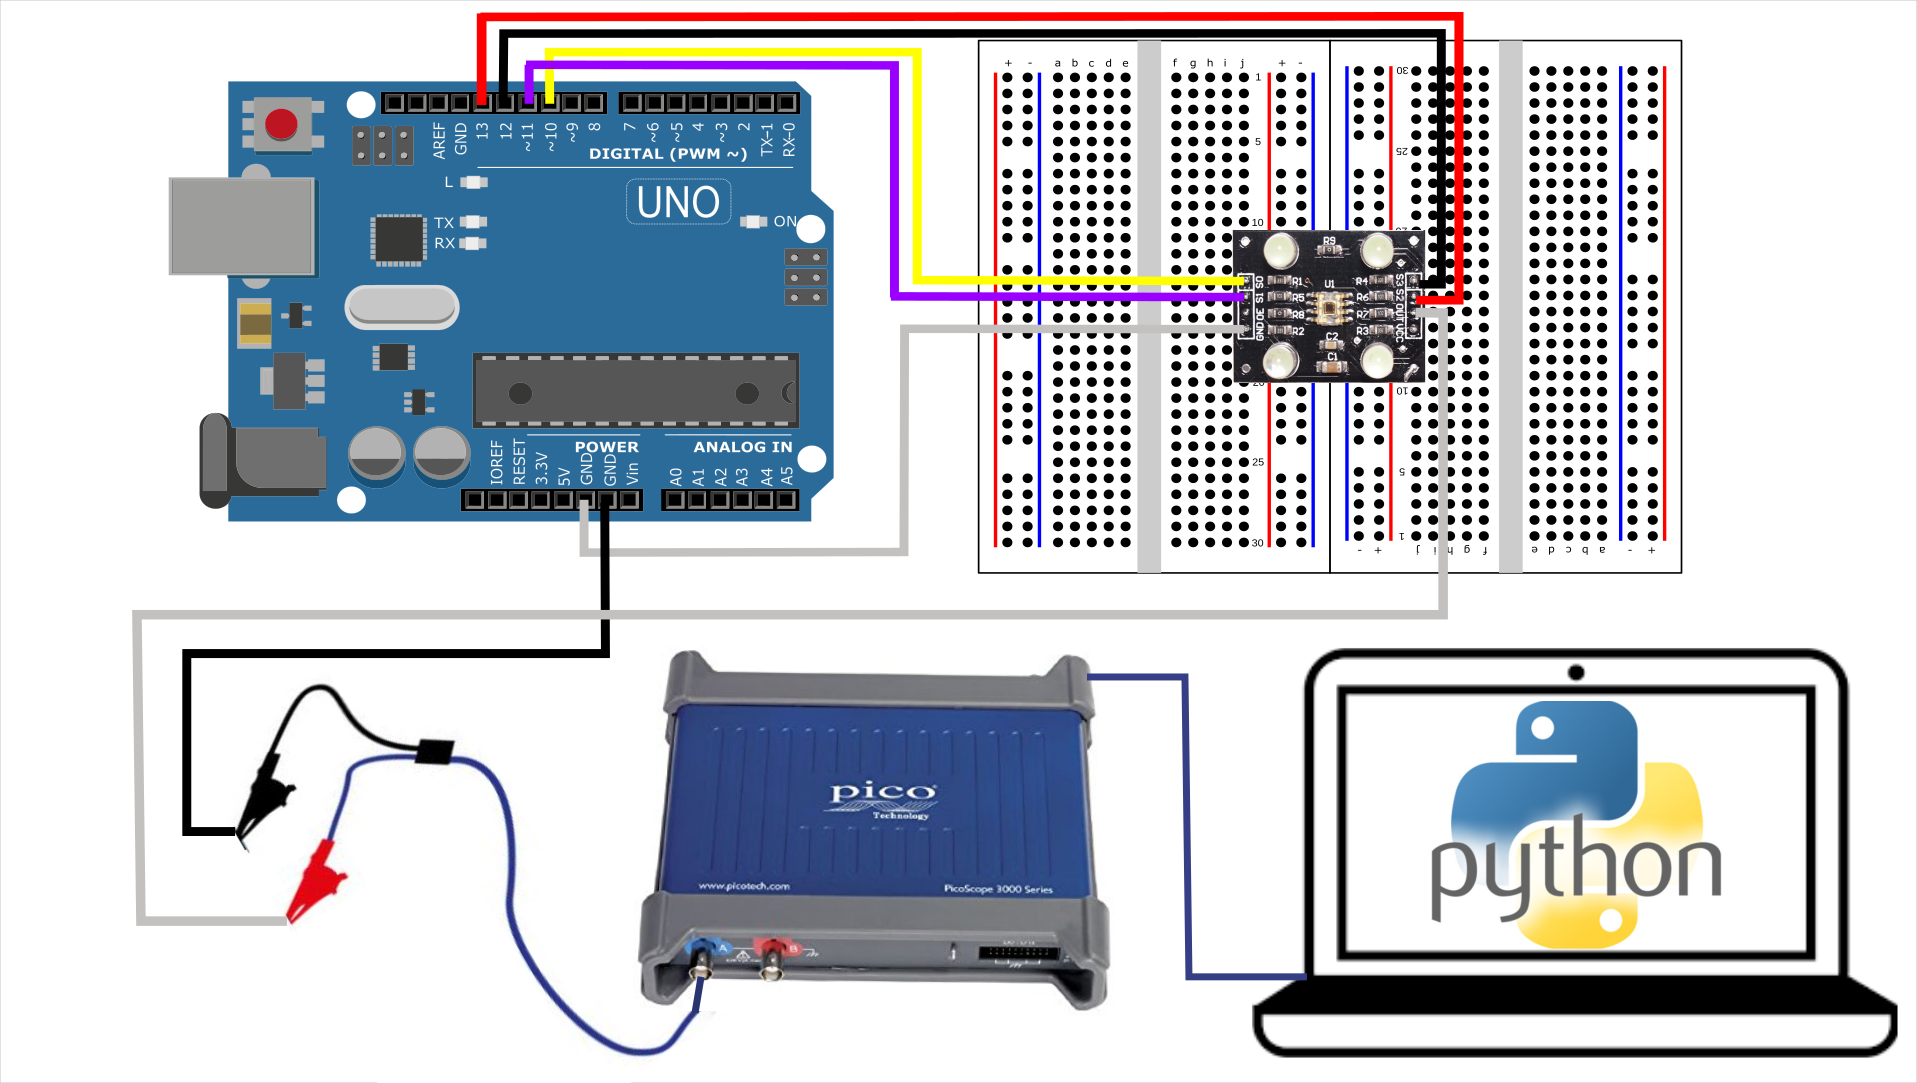
\includegraphics{img/experimental-setup_overview.png}
	\end{figure}
\end{frame}

\begin{frame}{Experimental Setup}
	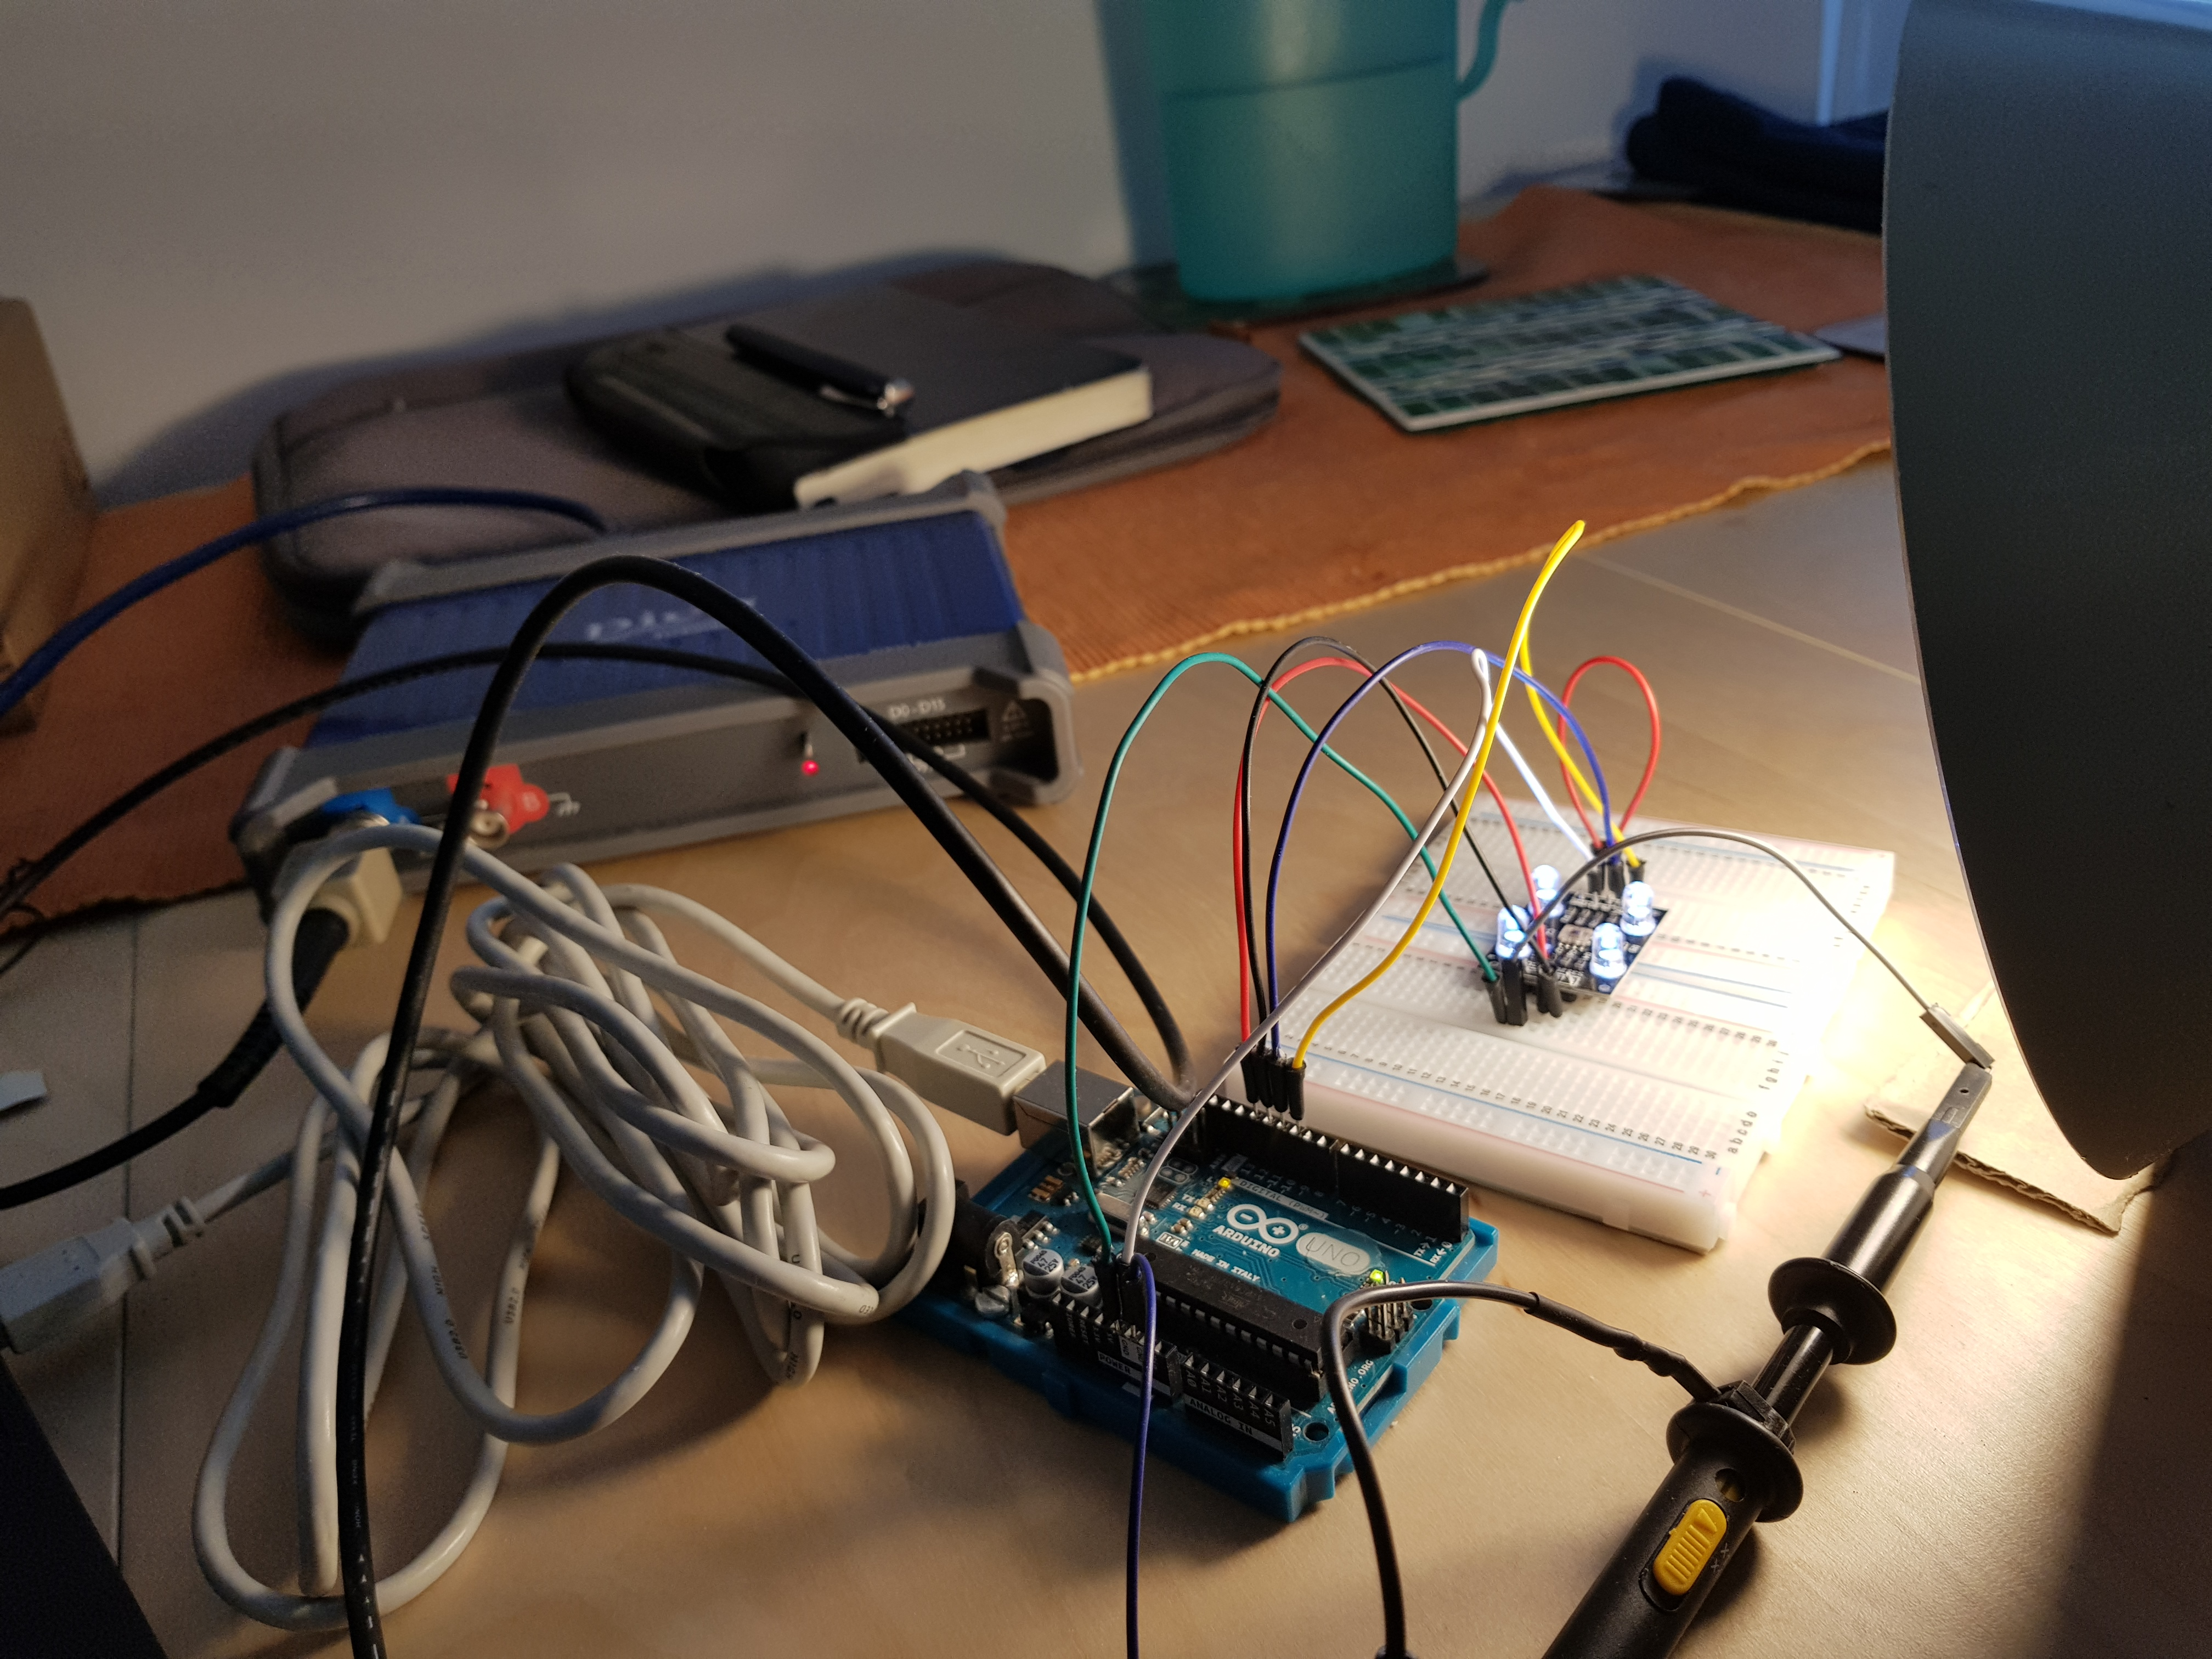
\includegraphics[trim={0 0 0 12cm},clip]{../experiment/project_setup/20180510_123244.jpg}
\end{frame}

\subsection{Results}%
\label{sub:results}

\begin{frame}{Some Results I} 
	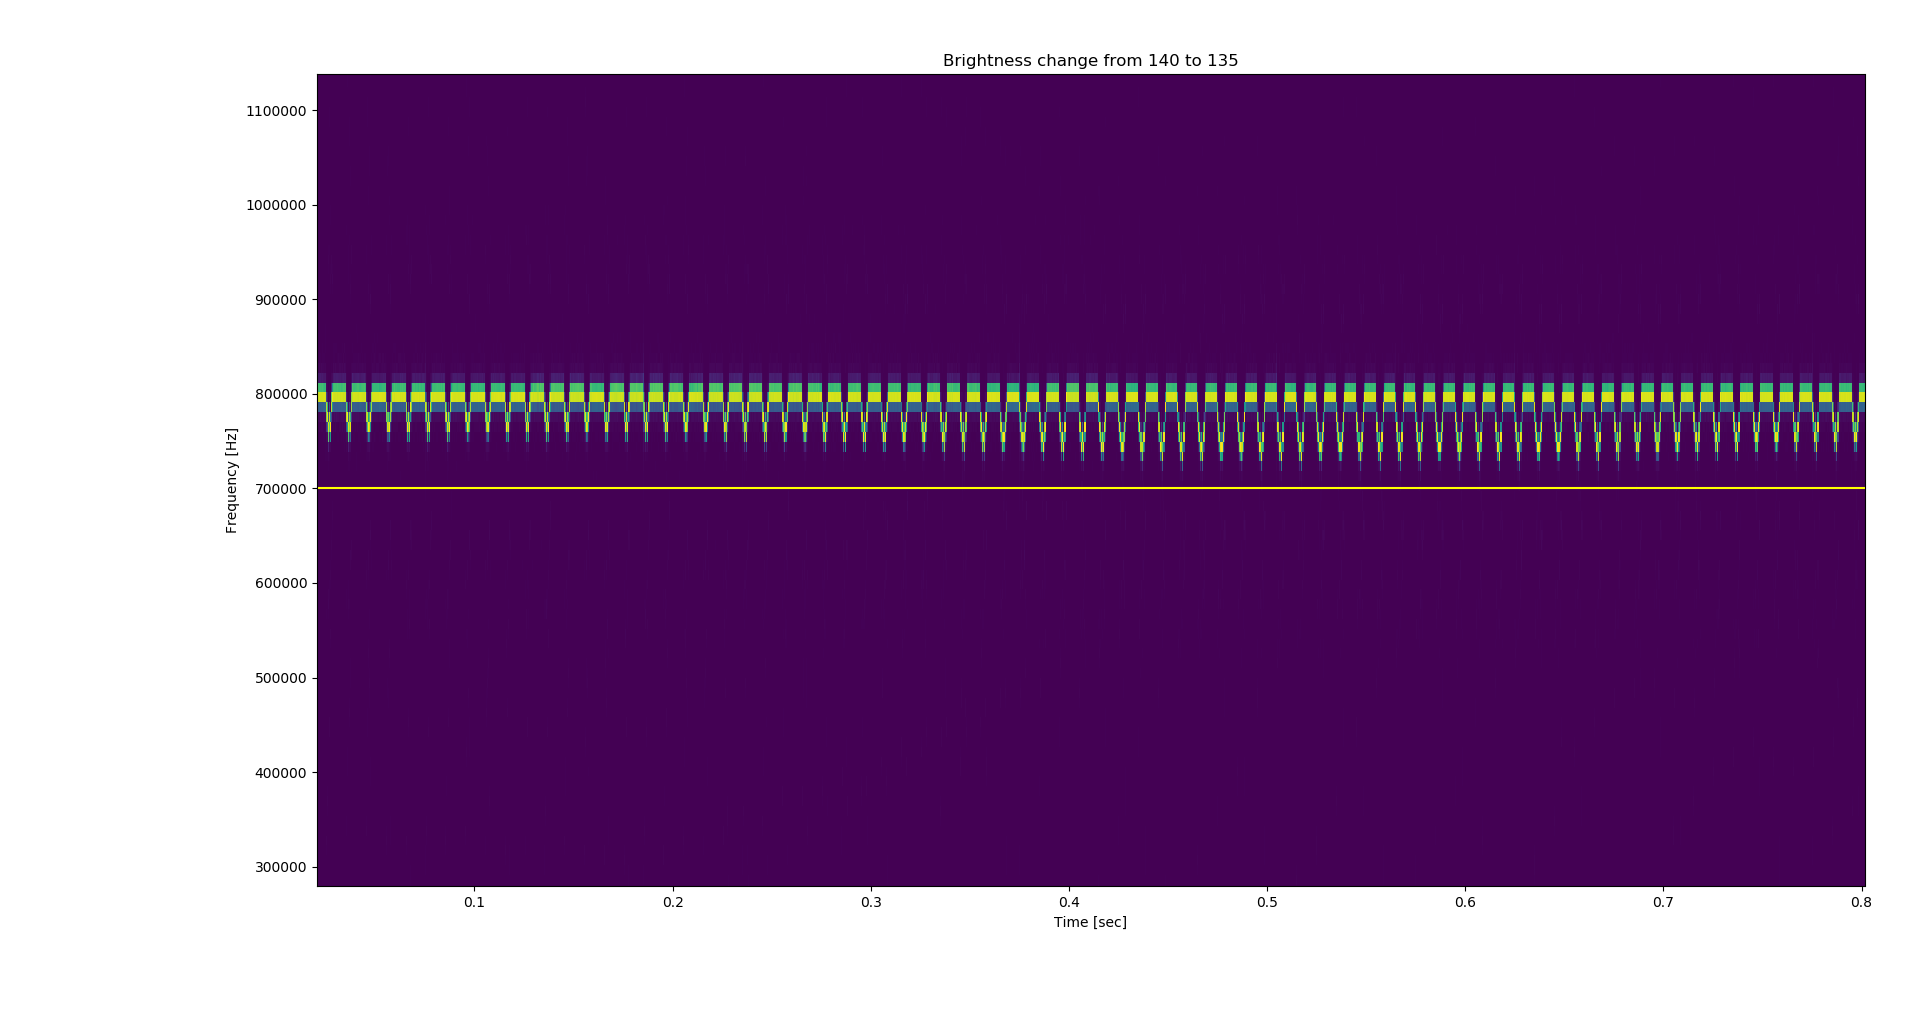
\includegraphics[width=\textwidth]{../experiment/140-135-2.png}
\end{frame}

\begin{frame}{Some Results II}
	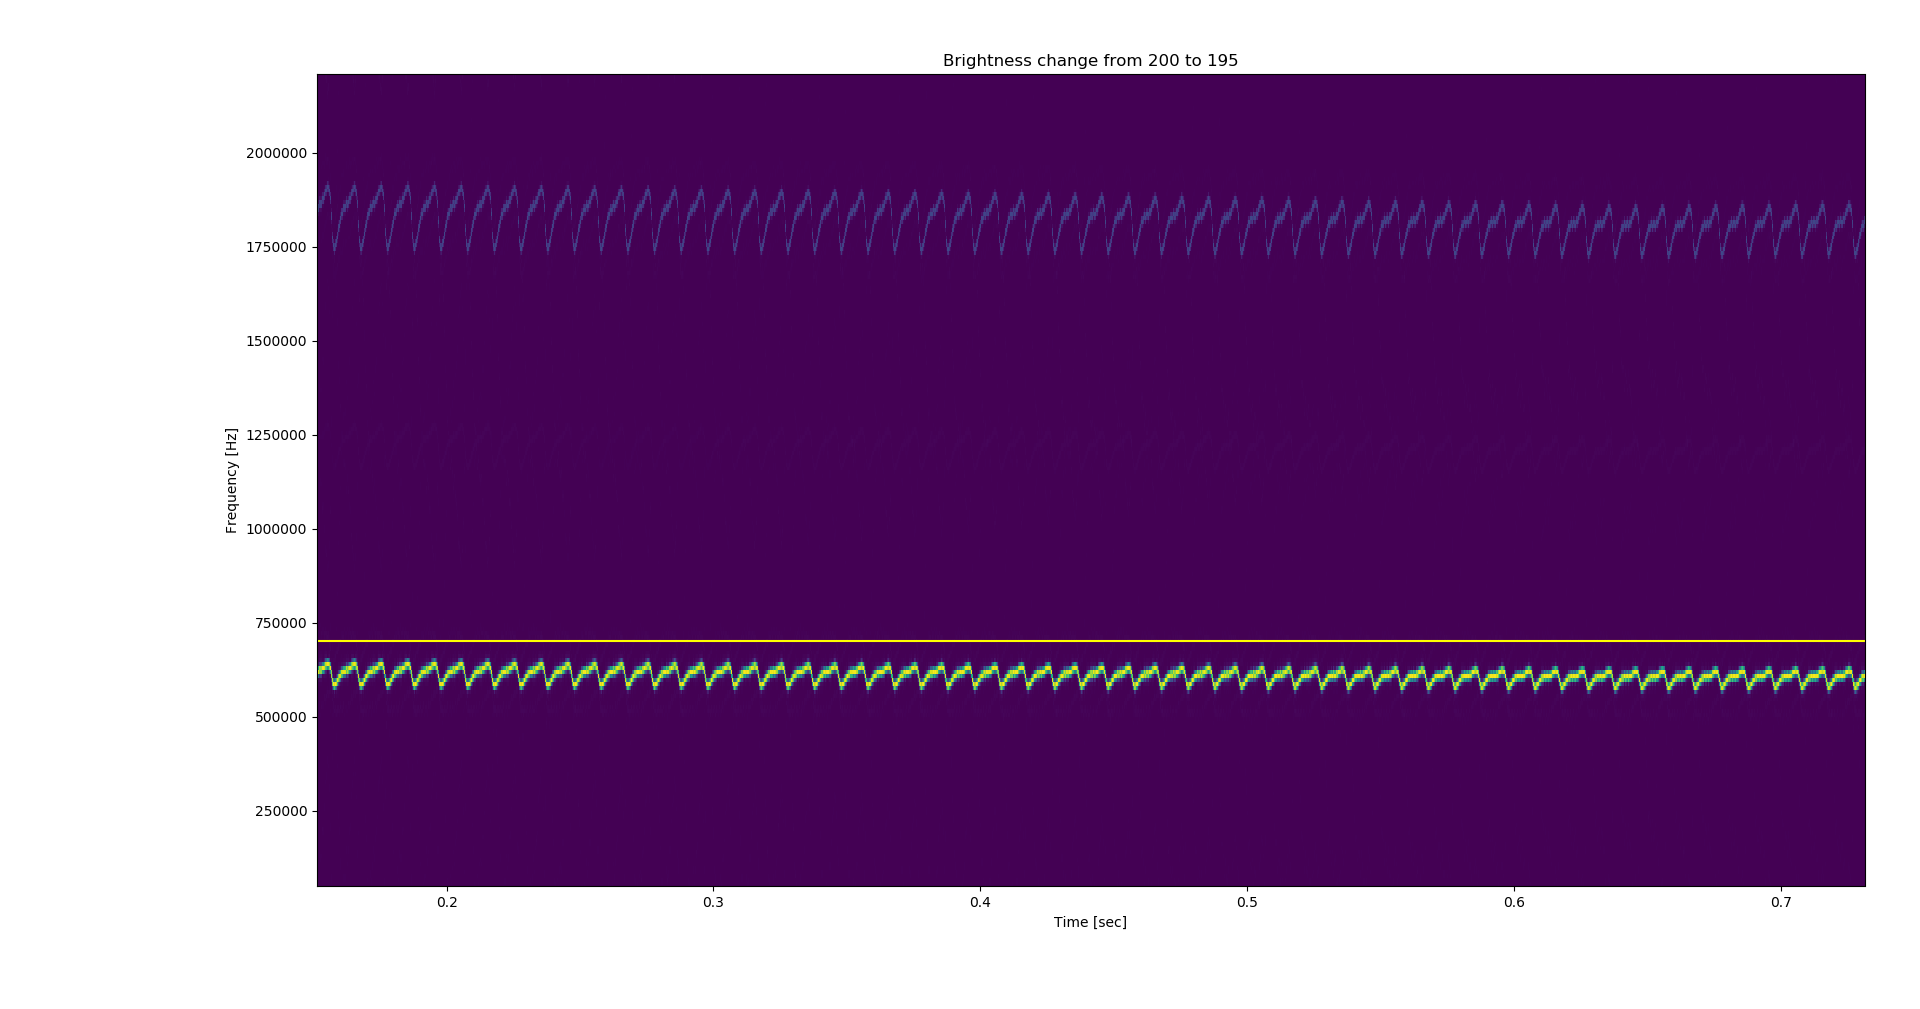
\includegraphics[width=\textwidth]{../experiment/200-195-10Mhz.png}
\end{frame}

\begin{frame}{Some Results III}
	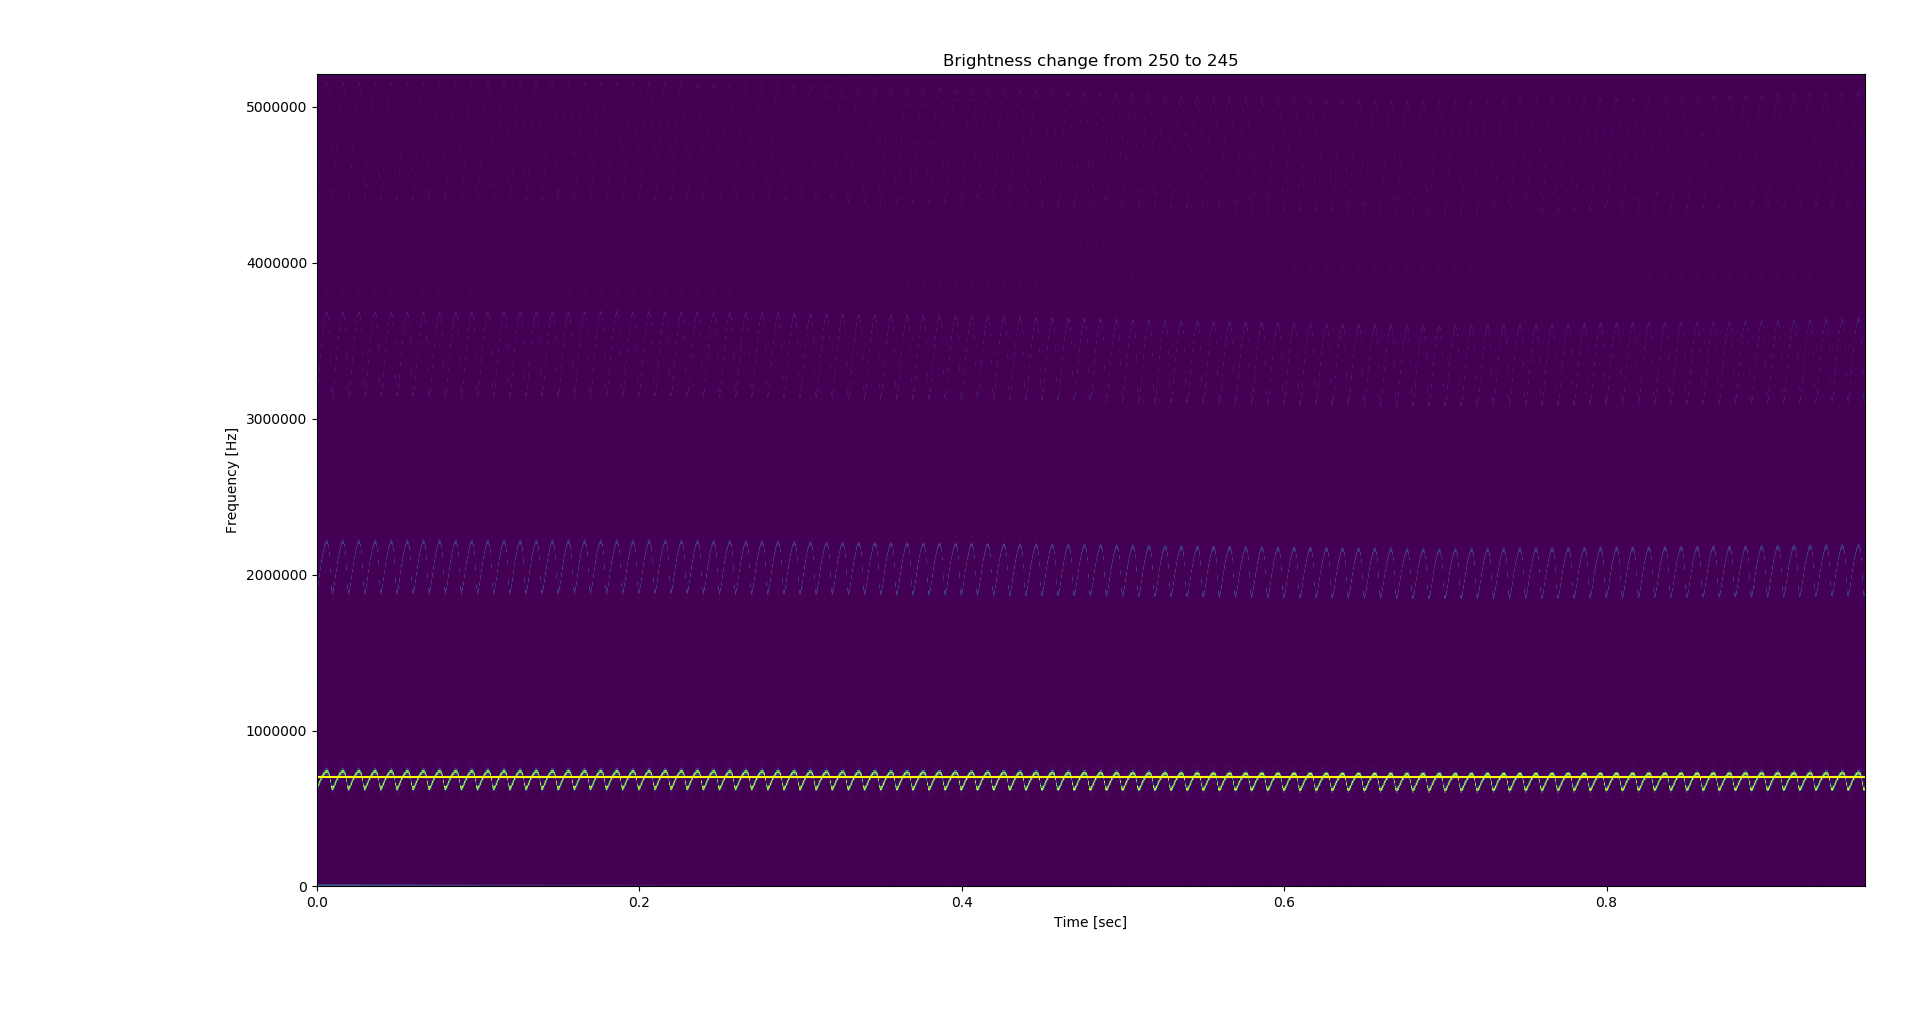
\includegraphics[width=\textwidth]{../experiment/250-245.png}
\end{frame}


\section{Demonstration} % 5 min
\label{sec:demonstration}
\title{Demonstration}
\subtitle{Covert Communication Channel on Philips Hue White Smart Light}


\section{Conclusion} % 3 min
\label{sec:conclusion}
\title{Conclusion}
\subtitle{Summary and Outlook}

\begin{frame}{Conclusion} % 1.5 min
	\begin{block}{Successes}
		\begin{itemize}
			\item We can distinguish brightness differences invisible to the human eye
			\item We \emph{think that we can} see the PWM, not just brightness
			\item TODO: Automatically detect brightness changes
		\end{itemize}
		$\rightarrow$ Research from \cite{Ronen:2016:EFAIDCSL} reproduced in principal.
	\end{block}

	\pause
	\begin{alertblock}{Failures}
		Automating this is hard:
		\begin{itemize}
			\item Very high variance in our measurements
			\item Much trial and error to obtain a good picture
			\item Limited range and robustness to lighting conditions
		\end{itemize}
	\end{alertblock}
\end{frame}

\begin{frame}{Outlook} % 1.5 min
	An automated covert channel could in principle be built using this technique.
	% TODO Good channel encoding, more robust pwm detection, higher range, automatic calibration needed of course!

	\begin{block}{Important Lessons}
		\begin{itemize}
			\item Connected LEDs should not be trusted in secure areas
			\item Smart lights should not have this many brightness levels. Fading and throttling improve their security a little though.
			\item Combine this demo with the insecurity of IoT devices for maximum effect.
			\item Alternatively, if you must use smart lights, isolate and secure them as much as possible.
		\end{itemize}
	\end{block}

\end{frame}



%% to show a last slide similar to the title slide: information for the last page
\title{Questions?}
\subtitle{}
\section{Questions}


%% appendix of 'extra' slides
\appendix

\begin{frame}[allowframebreaks]{Bibliography}
	\bibliographystyle{abbrvnat}
	\bibliography{../papers/literature.bib}
\end{frame}

\end{document}

% vim: spell ts=2 sw=2
